\section{Experimental Evaluation}\label{sec:evaluation}
\subsection{Design and statistical units}
The matrix-engine evaluation contains a 73-cell grid and six additional
long-stream runs: $176,520$ method-round records, with no full-product
discrepancy. Each cell uses five workload seeds and three repeats.
Per-update estimates take medians over rounds, repeats, then seeds;
speedups use within-seed ratios. Error bars are nominal $95\%$
percentile-bootstrap intervals from $2,000$ resamples of the five seed
summaries. Their small-sample resolution and shared-machine timing limit
population-level interpretation. Cumulative bands are pointwise and
include initialization. The extension reuses the same seeds and retains
its separate estimates. The connected study uses twenty same-tape pairs
for $q=17$ replay, twenty fresh source-paired streams per encoding for
$q=65521$ service, and twenty independent utility simulations, displaying
the individual units and full view diagnostics in the supplement.

The fixed Covertype extension uses $b=8,t=2,k=256$ at
$n\in\{256,512,1024\}$ on server GPU2 and $n\in\{512,1024\}$ on a
Spark CPU, plus one synchronized $n=1024$ diagnostic. Jobs run
sequentially within each host. The artifact preserves the full grid,
source identities, seed summaries, setup costs, and timing boundaries.
The code and lightweight reproducibility materials are available at
\footnote{\url{https://github.com/fuyuefyu/verifiable-matrix-maintenance}}.

\subsection{Strength of the bounds}
Figure~\ref{fig:theory-bounds}(a) compares the work profile with both
the combined slice/geometric-rank and exact-zero-probability range bounds. The positive
budget $w=56$ example improves the latter by approximately
$9.95\times10^4$, locating the gain in rank conditioning rather than
zero-work agreement. Composition also changes the certificate:
at $n=4,r=2,q=2,k=4,W=8,t=1$, the refined bound is $0.115421$ versus
the threshold bound $0.586182$, even though no round can reach $R_0=16$.

Exact enumeration validates the rank formula on $417$ matrices,
profile allocation on $7,294$ comparisons, and balanced allocation
on $360$ comparisons. The heterogeneous allocator agrees across
$15,147$ configurations and $1,651,995$ candidate comparisons,
including $3,360$ cases with tied optima. Its grid covers
$q\in\{2,5,17\}$, $k=2,\ldots,5$, $T=k,\ldots,k+8$, and
$b=0,\ldots,k-1$, with uniform, mixed, and endpoint profiles.
The single-round witness is checked on $794,884$ input pairs and
$19,651,396$ explicit checking vectors over fields of size two, three,
and five. These are evaluations of mathematical bounds and procedures,
not measured attack probabilities.

\begin{figure*}[t]
  \centering
  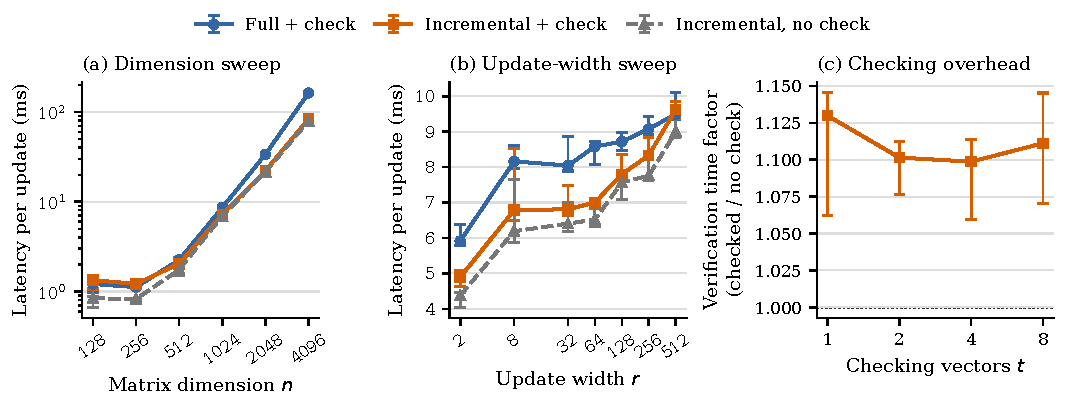
\includegraphics[width=\textwidth]{figures/engine_scaling.pdf}
  \caption{End-to-end matrix-maintenance latency and checking overhead across matrix sizes and update widths.}
  \label{fig:engine-scaling}
\end{figure*}


\subsection{Complete-update benefits and bottlenecks}
At $n=4096,r=8,t=2$, checked GPU maintenance takes $83.162$\,ms
against $161.931$\,ms for checked recomputation, a paired speedup of
$1.947\times$ ($[1.931,1.985]$). The width sweep reaches $1.968\times$
at $r=32$ and falls to parity at the largest widths. The complete
pipeline's checking factors for $t=1,2,4,8$ are
$1.130,1.101,1.099,1.111$; shared candidate costs prevent a linear
extrapolation; the full scaling sweep is shown in Figure~\ref{fig:engine-scaling}.

The structured Covertype view gives a second reuse regime, with the full
diagnostic retained in the supplement. At $n=1024,b=8$, GPU incremental latency
is $4.463$\,ms versus $5.712$\,ms, a paired $1.279\times$ gain
($[1.227,1.280]$). The CPU extension reaches $2.098\times$
($[2.086,2.112]$). Detailed cache diagnostics, device-specific intervals,
and setup-inclusive stage timings are reported in the supplement and
remain in the artifact.

\subsection{Encoding and checking choices for randomized views}
\label{sec:connected-results}
The categorical view connects a report-encoding choice to an accuracy
requirement and a fresh-work target on a $40\times40$ domain, with
privacy-matched SUE and OUE. Utility uses twenty independently
simulated randomizations at four nested source prefixes, with common
random numbers between the privacy-matched encodings within a replicate.
The performance comparison uses twenty shared report tapes per policy;
the live-service runs instead generate new operating-system report coins
after each fixed program. Replaying a tape contributes no new fresh-work
episode. Utility simulations and small-field replays are distinct from the
fresh-input integrity-service runs.

\paragraph{Statistical accuracy}
Figure~\ref{fig:application-results}(a,b) evaluates all 1,600 cells and
the twenty cells selected by the true full-data counts before examining
noisy estimates; all estimates are unclipped. With $N$ the number of
source records and $H$ the true count table, frequency mean squared error
(MSE) is $n^{-2}\|\widehat H/N-H/N\|_F^2$, with $\|\cdot\|_F$ the
Frobenius norm. Panel~(a) places the four nested source prefixes at equal
horizontal spacing, shows all twenty replicate frequency root mean squared
error (RMSE) values, and draws solid curves as the root mean MSE, the
square root of the mean replicate MSE, and dashed curves as
$\sqrt{\E[\mathrm{MSE}]}$. For a single-parameter stratum, write $p$ and
$\beta$ for the common $p_j$ and $\beta_j$, and put
$\sigma_0^2=\beta(1-\beta)/(p-\beta)^2$ and
$\sigma_1^2=p(1-p)/(p-\beta)^2$. Independence of attribute noises makes
the sum of cell variances per record
$[(n-1)\sigma_0^2+\sigma_1^2+1]^2-1$, regardless of its categories.
For the equal parameter strata, the whole-table frequency MSE therefore
satisfies
\[
 \E[\mathrm{MSE}]_{\rm SUE}=\frac{47}{20N},\qquad
 \E[\mathrm{MSE}]_{\rm OUE}=\frac{1925689}{1036800N}.
\]
Panel~(b) draws one line per replicate pairing SUE and OUE at
$N=581{,}012$ on the twenty cells selected by the true full-data counts,
with fixed tie breaking, and marks the median frequency RMSE in black.
Across all four prefixes and both encodings, empirical mean MSE is within
$0.8\%$ of its analytical value. At $N=581{,}012$, the whole-table root
mean MSE is $2.018\times10^{-3}$ for SUE and $1.781\times10^{-3}$ for OUE:
their ratio is $1.133$ with nominal interval $[1.123,1.142]$.
The median paired top-twenty RMSE ratio is $1.138$ ($[1.046,1.357]$).
Thus SUE's stronger work certificate in this application accompanies
about $13\%$ higher whole-table root mean MSE; the two encoding choices
expose a quantifiable accuracy--work-guarantee tradeoff.

\paragraph{From a target to measured checking cost}
At $q=17$, with $k=512$ and $r=2$, the exact allocator (OPT) certifies
the minimum of $767$ checks for $\delta=(31/50)^{64}=5.165\times10^{-14}$. Certificate-marginal
greedy starts with $t_j=1$ and repeatedly maximizes
$\log\Psi(\mathbf t)-\log\Psi(\mathbf t+\mathbf e_j)$, where
$\mathbf e_j$ is the $j$-th standard unit vector, breaking ties by fixed
index. It reaches the same $767$-check schedule here; fixed-prefix round
robin (RR) requires $856$. Adapting checks to the round parameters
therefore saves $10.4\%$ relative to RR. The preceding
budgets $766$ and $855$ fail the corresponding exact target tests.
Theorem~\ref{ext:thm-heterogeneous} provides the general global-optimality
guarantee. The specialized procedure agrees with exhaustive enumeration
on $162$ small cases ($6,804$ allocations) and $56$ full-size comparisons.

Observed complete plan-generation charges are $3.473$ and $2.743$\,ms
for OPT and RR. A separate matched search-only comparison on fy,
using five blocks with rotating policy order, gives medians
 $1.553$, $0.866$, and $34.443$\,ms for OPT, RR, and certificate-marginal
greedy, using cached coefficients and incremental certificate evaluation.
These spans exclude serialization and output validation;
the service comparison below retains the complete plan-generation charges.

We charge the complete fy plan-generation cost once per twenty-session
batch. Service execution runs separately on the ebaf CPU; each stream
includes plan reading, initialization, complete candidates, sequential
checks, and decoding. Figure~\ref{fig:application-results}(c) uses twenty
CPU replay pairs from this service and allocates the measured
plan-generation charge equally across sessions. For policy
$a\in\{\mathrm{RR},\mathrm{OPT}\}$, let $\tau_a$ denote measured service
time, and let $\pi_a$ denote the plan-generation time; the charged ratio is
$(\tau_{\rm RR}+\pi_{\rm RR}/20)/(\tau_{\rm OPT}+\pi_{\rm OPT}/20)$. Reported
intervals are nominal $95\%$ paired percentile-bootstrap intervals over
twenty replicate or stream IDs within each experiment; the intervals in
(a) preserve the nested prefixes and are pointwise. The median paired
ratio is $1.0233$ with nominal interval $[1.0207,1.0254]$; the twenty-session
service-plus-planning totals are $997.488$\,ms for RR and
$983.342$\,ms for OPT. Nineteen of twenty CPU pairs favor OPT; the
remaining ratio is $0.869$, so the full-batch saving is $1.4\%$.
The corresponding GPU paired ratio is $1.0459$
($[1.0417,1.0590]$), and the batch ratio is $1.0482$.
These intervals condition on the observed planning cost and shared-machine
schedule. These $q=17$ policies are matched on the work target; their
output-integrity certificates differ.

\paragraph{Fresh-input service at the integrity setting}
At $q=65521$, impose the common integrity certificate
$I(\mathbf t)\le\varepsilon=512/q^2=1.193\times10^{-7}$.
Since $q>512$, one round with $t_j=1$ already exceeds this budget.
Thus every round needs at least two checks and $T\ge1024$.
For SUE, $\kappa=1/8$ and
$f_{\rm SUE}\exp(\varepsilon/8)<\delta$; by
\eqref{eq:integrity-work-link}, uniform $t=2$ attains the minimum
$T=1024$ under both certificates. Its work bound is
$1.893\times10^{-14}$. OUE's floor $4.105\times10^{-4}>\delta$
precludes this work target through the threshold certificate.
Here integrity determines the checking count, while encoding determines
work-target feasibility. These are analytical certificates under the
stated hypotheses, not measured attack rates.
Table~\ref{tab:connected-live} reports twenty fresh streams per encoding
and backend on the Spark-ebaf CPU and fy's RTX~5090 GPU0, with $q=65521$
and median milliseconds per 512-round stream. Live time is the continuous interval including report
generation; active time removes measured client-generation spans and is
a discontinuous subtotal. All $160$ replay/live streams complete their $512$ rounds
and their final decoded arrays match direct integer reconstruction from
the reports. At this $40\times40$ size, the tested ebaf CPU is the
lower-latency choice than fy's RTX~5090 GPU0; GPU per-round transfers
and kernel launches remain visible
in the complete candidate interface.

\begin{table}[t]
\caption{Median live and active service latency in milliseconds for 512-round fresh-input streams.}
\label{tab:connected-live}
\centering
\begin{tabular}{llrr}\toprule
Backend & Encoding & Live time & Active time\\\midrule
CPU & SUE & 65.289 & 51.773\\
CPU & OUE & 64.445 & 51.592\\
GPU & SUE & 627.120 & 589.921\\
GPU & OUE & 624.246 & 588.208\\\bottomrule
\end{tabular}
\end{table}

